\subsection{Styr- och reglersystem}
\label{subsec:styr och regler}
För att styra svävaren samlas acclerometerdata in i realtid på fjärrkontrollen.
Dessa processeras sedan och omvandlas till styrsignaler som skickas till
Routern. På Routern passerar signalerna genom reglersystemet för att sedan
skickas som motorstyrsignaler till ADKn.där det även finns plats för ett
reglersystem.

\subsubsection{Styrsystem}
Systemet för att implementera styralgoritmer är uppbygt kring designmönstrena
Composite \cite{Composite pattern} och Builder \cite{Builder pattern}. Detta gör
det enkelt att implementera olika styralgoritmer.

Man kan genom dropdown listor på fjärrkontrollen välja vilken styralgoritm som
ska användas. De olika styralgoritmerna utvecklades med hjälp av MATLAB för att
sedan implementeras i Java på fjärrkontrollen. De olika styralgoritmernas utslag
då pitch = 30\degree  då roll går från -45\degree till 45\degree  kan ses i
figur~\ref{fig:styralgoritmer}.

\begin{figure}[htbp!]
\centering
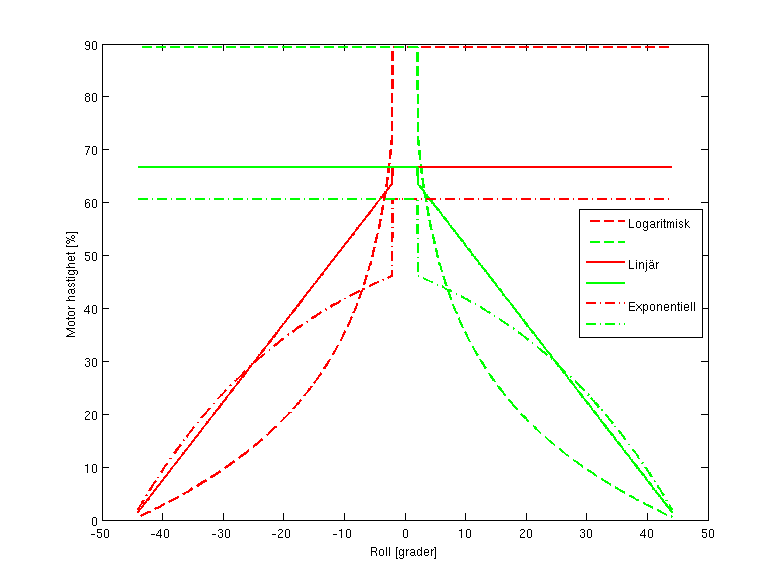
\includegraphics[width=12cm]{../../includes/figures/Styralgoritmer}
\caption{Styralgoritmernas utslag vid pitch = 30\degree då roll = [-45,45].}
\label{fig:styralgoritmer}
\end{figure}

\subsubsection{Reglersystem}
Designen av svävaren medförde starkt korskoppling mellan hastighet och
styrning vilket medför svårigheter då en regulator ska implementeras.
Grundlig efterforskning gjordes och det bestämdes att ramverket ACADO
\cite{ACADO} skulle användas för att implementera en regulator till svävaren då
ramverket kunde autogenerera kod för mer komplexa regulatorer. Detta visade sig
vara svårare än förutspått och ramverket krävde även mer minne än vad som fanns
tillgängligt. Dessa bakslag medförde att reglersystemet lades på is för att
kunna vidareutvecklas vid ett senare tillfälle.

\subsubsection{Resultat}
Det implementerades fyra olika implementationer av styralgorithmer för att
processea pitch- respektive rolldata. I realiteten märkte föraren dock ingen
större skillnad mellan de olika styrlägena. Styralgoritmerna processerar
acclerometerdatan på liknande sätt men med olika matamatiska funktioner, de tre
lägena är logaritmisk, exponentionell och linjär.

Implementationen av reglersystemet är bara ett tomt skal. Den funktionallitet
som han implementeras var enbart vidarebefodring av styrsignaler till ADKn.

\subsubsection{Vidareutveckling}
Endast styrning via proccesering av accelerometerdata implementerades och det
hade varit intressant att se hur det hade förändrats om man hade implementerat
en mer klassisk fjärrkontroll via den tryckkänsliga skärmen.
